\documentclass{jfsma}
\usepackage{lmodern}
\usepackage{hyperref}
\usepackage{caption}
\usepackage{cuted}
\usepackage{etoolbox}

\titre{Automatic Observer For Real-Time Strategy Games} % On garde ce titre ?
\auteur{Emmanuel \textsc{Hadoux}}{emmanuel.hadoux@lip6.fr}
\auteur{Thomas \textsc{Huraux}}{thomas.huraux@lip6.fr}
\institution{
  Sorbonne Universit\'es, UPMC Univ Paris 06, CNRS, LIP6 UMR 7606\\4 place Jussieu 75005 Paris}

\begin{document}
\maketitle

\begin{strip}
  \centering\noindent
  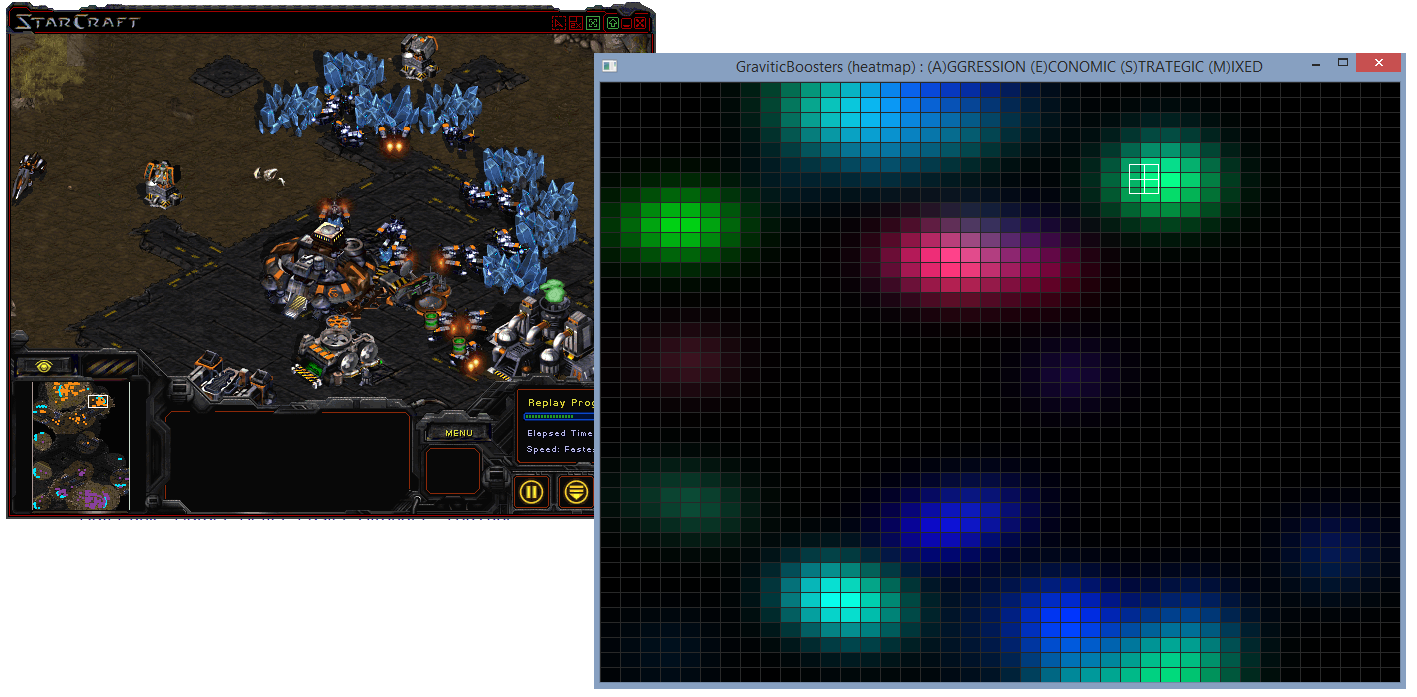
\includegraphics[scale=0.28]{gfx/GB}
  \vspace{0.3cm}
\end{strip}

	\section{Context}
    Electronic sport (\textit{e-sport}) is a not-so-young discipline slowly growing in western countries~\cite{taylor2012raising}.
    It took root in South-Korea about 15 years ago and is currently experiencing an explosion of interest.
    The first game entering the closed category of e-sport was StarCraft 1. % T: faut voir si on parle tout de suite de SC ou alors on vise un truc plus générique
    This fast-paced real-time strategy game (\textit{RTS}) was released in 1998.
    Since then RTS games have challenged many research works in AI such as planning in resource allocation, force deployment, and battle tactics~\cite{weber2009case,mccoy2008integrated}; spatial reasoning~\cite{forbus2002qualitative} or opponent modeling~\cite{schadd2007opponent}.

    During battles between armies, players can reach peaks of 450 actions-per-minutes.
    For this obvious reason, viewers cannot follow the game by watching the screens of the players.
    Competitions thus require an external observer following the game and showing important actions.
    However, being an observer requires a comprehensive knowledge of the game as well as anticipation and entertainment faculties.
    Few persons are able to gather those skills, making them more famous than some professional players.

    In this work, we propose an automatic observer able to catch every piece of action to assist or replace the human observer. The following section briefly describes our approach to answer this problem.

\section{Overview of the method}
We set ourselves two constraints to the realization of an automatic observer: on the one hand real time calculation to be used in the context of a game with pro players, and on the other hand, to use only standard information that can be found in any RTS (position, unit price, damage, ...).
As far as we know, no previous research work have been made on this topic in the video game context.
Nevertheless, we found on TeamLiquid (a famous website about StarCraft) an attempt to automatically product Youtube videos from finished game logs\,\cite{tl}.
However, this solution is based on simple \emph{ad-hoc} rules and thus is only appliable to StarCraft 1.
Our objective is to remove this assumption even though few games can be linked to user code due to legal issues.

In our model, each entity has 3 potentials computed in real time:\\
\textsc{aggressive potential} allows to anticipate the interest of an upcoming fight by taking into account the distance to the enemy and the damage per second\\
\textsc{economic potential} informs on base creation, workers training, etc.\\
\textsc{strategic potential} shows information-taking units (called \emph{scoot})

Those 3 features are the most important sides of a competitive RTS game.
Indeed, players need workers and bases to gather resources allowing them to build an army.
However, as they cannot train workers and units at the same time, they need to choose to go agressive or economic based on gathered strategic information.
The purpose of this model is to show where and when those choices are made and thus complementing the work of the casters (the commentators).
To this end, the map is discretized so that each cell aggregates the potentials of all entities composing it.
The camera is then positioned at the maximum value of the resulting matrix.
To adjust the positioning to the action, we smooth the potential matrix using a gaussian kernel.
This allows, for instance, to position the camera between two armies facing each other.
We also added two dynamic parameters to the camera: \emph{commitment} and \emph{weariness} in order to limit both too-frequent disturbing changes and over-attention to the same area.

\section{Implementation}

Based on this method, we develop an automatic observer called \emph{Gravitic Boosters}\,\footnote{\url{http://github.com/EHadoux/GraviticBoosters}}.
We tested our approach on StarCraft BW\,\footnote{\url{http://us.blizzard.com/en-us/games/sc/}} using
the BWAPI API~\cite{bwapi} which enables to retrieve all live information and take control of both the units and the game interface.
As a side note, this API has been used for 5 years in several StarCraft AI Competitions, supported by the University of Alberta\,\footnote{\url{http://webdocs.cs.ualberta.ca/~cdavid/starCraftaicomp/}}. % TODO Revoir cette phrase (cf review 3)

The figure above shows a StarCraft game and a corresponding visualization of the 3 potentials as a heat map.
RGB colors are used to encode the 3 components: red represents the aggressive potential, green the economic potential and blue the strategic one.

\section{Perspectives}
With all the potentials computed for each tile, it would be interesting to analyze the points generated.
In fact, we can see that, depending on the type of the tile (main base, first expansion, attack path, etc.) we can clusterize the points.
The clusters can act as a profil for a tile, that can be learn and used online, while observing the game, to explain what is happening.
%We consider several perspectives in the context of this work in order to increase the accuracy of our observer.
%Firstly, we plan to take into account the spaciality of the events (unit creations, skirmishes, \emph{etc.}). % TODO Expliquer ou enlever
%Self-Organizing Maps seem very adapted for such a purpose.
%Secondly, we could use clusterization to group similar game sequences.
%This will allow the automatic observer to not only follow the action, but also explain what it is going on.
%Those two perspectives are works in progress.

The video game industry continues to expand while almost no AI has been involved in this expansion~\cite{miikkulainen2007creating}.
Unfortunately, AI seems not to be a priority of publishers compared to \textit{e.g.} graphics with a better marketing value.
Nevertheless, we believe that AI can bring more to this media.
We try to illustrate this point with our work presented in this paper.
Recent competitions with over 10.000.000\$ in prize money and stadiums under construction are among indicators that video games and e-sport especially provide real life applicated research opportunities.
We argue that such research should be encouraged to take advantage of this recent expansion.

\bibliographystyle{plain}
\bibliography{biblio}

\end{document}
